% !Mode:: "TeX:UTF-8"

% Latex template for Foreign Language Translation from University of South China.
% Author: Zhu Liucheng
% E-mail: 2576950110@qq.com
% Date : 2022/3/7

\documentclass[a4paper,onecolumn,12pt]{translation}
% a4paper 用a4纸张大小
% onecolumn 单排 亦可以使双排 twocolumn
% 10pt 11pt 12pt
% article 文档样式,report book slides

\usepackage{style/translationstyle} % 引用自定义布局

\begin{document}
%header
%---------------------------------------------------------------------
%	封面设置
\renewcommand\arraystretch{0.8} % 表格行间距

\begin{titlepage}
  \begin{center}
    
\includegraphics[width=0.8\textwidth]{logo.png}\\
    \vspace{30mm}
    \textbf{\zihao{2}{\heiti{毕业论文/设计外文翻译}}}\\[0.8cm]
    \vspace{40mm}
  
    \begin{center}
    	\begin{large}
    		\begin{tabular}{rc}
    			\bfseries \fs{\xiaoerhao{题\qquad 目}}& \hspace{1.7cm}\xiaoerhao{\fs{对深度学习的几何理解\hspace{1.7cm}}} \\
    			\cline{2-2}\\
    			\xiaoerhao{\fs{学院名称}}& \xiaoerhao{\fs{数理学院}}\\
    			\cline{2-2}\\
    			\xiaoerhao{\fs{指导老师}}& \xiaoerhao{\fs{高有}}\\
    			\cline{2-2}\\
    			\xiaoerhao{\fs{职\qquad 称}}& \xiaoerhao{\fs{讲师}}\\
    			\cline{2-2}\\
    			\xiaoerhao{\fs{班\qquad 级}}& \xiaoerhao{\fs{信计1802}}\\
    			\cline{2-2}\\
    			\xiaoerhao{\fs{学\qquad 号}}& \xiaoerhao{\fs{20184390213}}\\
    			\cline{2-2}\\
    			\xiaoerhao{\fs{学生姓名}}& \xiaoerhao{\fs{朱柳承}}\\
    			\cline{2-2}
    		\end{tabular}
    	\end{large}

      \vspace{13mm}
      \erhao{\fs{2022年1月15日}}

    \end{center}
    \vfill \hfill
  \end{center}
\end{titlepage}

%-------------------------------------------------------
% Contents
% \newpage \tableofcontents \newpage
% \setcounter{page}{1}
% \rhead{Page \thepage\ of \pageref{LastPage}}

%summary
%---------------------------------------------------------------------------%
%->> Identification
%---------------------------------------------------------------------------%
\ProvidesFile{summary.cfg}[2014/10/01 v1.0 class configuration file]%
%---------------------------------------------------------------------------%
%->> Labels in Chinese titlepage
%---------------------------------------------------------------------------%
\def\usc@label@ch@thesis{毕业论文文献综述}
\def\usc@label@ch@title{题\quad\quad 目}
\def\usc@label@ch@author{学生姓名}
\def\usc@label@ch@authorid{学\quad\quad 号}
\def\usc@label@ch@advisor{指导教师}
\def\usc@label@ch@advisortitle{职\quad\quad 称}
\def\usc@label@ch@degree{学位类别}
\def\usc@label@ch@major{班\quad\quad 级}
\def\usc@label@ch@field{研究方向}
\def\usc@label@ch@institute{学院名称}
\def\usc@label@ch@date{填表日期}
\def\usc@label@ch@mark{2022年1月30日}
\def\usc@value@ch@date{\the\year~年~\ifnum\the\month <10 0\fi\the\month~月}
%---------------------------------------------------------------------------%
%->> Structure elements
%---------------------------------------------------------------------------%
\def\usc@label@ch@tocname{目\quad\quad 录}
\def\usc@label@en@tocname{Contents}
\def\usc@label@ch@lsfigname{图形列表}
\def\usc@label@en@lsfigname{List of Figures}
\def\usc@label@ch@lstabname{表格列表}
\def\usc@label@en@lstabname{List of Tables}
\def\usc@label@ch@algname{算法}
\def\usc@label@en@algname{Algorithm}
\def\usc@label@ch@bibname{参考文献}
\def\usc@label@en@bibname{References}
\def\usc@label@ch@bibetal{等}
\def\usc@label@en@bibetal{et al.}
\def\usc@label@ch@biband{和}
\def\usc@label@en@biband{ and }
\def\usc@label@ch@axiomname{公理}
\def\usc@label@en@axiomname{Axiom}
\def\usc@label@ch@theoremname{定理}
\def\usc@label@en@theoremname{Theorem}
\def\usc@label@ch@lemmaname{引理}
\def\usc@label@en@lemmaname{Lemma}
\def\usc@label@ch@corollaryname{推论}
\def\usc@label@en@corollaryname{Corollary}
\def\usc@label@ch@assertionname{断言}
\def\usc@label@en@assertionname{Assertion}
\def\usc@label@ch@propositionname{命题}
\def\usc@label@en@propositionname{Proposition}
\def\usc@label@ch@conjecturename{猜想}
\def\usc@label@en@conjecturename{Conjecture}
\def\usc@label@ch@definitionname{定义}
\def\usc@label@en@definitionname{Definition}
\def\usc@label@ch@examplename{例}
\def\usc@label@en@examplename{Example}
\def\usc@label@ch@remarkname{注}
\def\usc@label@en@remarkname{Remark}
\def\usc@label@ch@proofname{证明}
\def\usc@label@en@proofname{Proof}
\def\usc@label@ch@keywords{关键词:}
\def\usc@label@en@keywords{Keywords:}
%---------------------------------------------------------------------------%
\endinput



%-------------------------------------------------------
% Main Body
% !TeX root = ../uvanode.tex

\section{项目简介}

多智能体系统是指由多个机器人(无人机)通过分布式的协同控制形成统一行为的系统,具有单个智能体无法比拟的优势,在诸如战地环境探测,灾难救援、污染防治等方面用着广泛的应用。本项目将以多智能体系统的集群性的理论研究及其在多无人机直线编队为主要研究内容,对编队形成的时间上限估计是与初始状态之间的内在联系等问题开展研究和数值仿真,实现对多无人机直线编队的人为控制。本项目的研究内容不仅在发展多智能体复杂系统的新理论和新方法方面具有重要意义,而且对多无人机在有限时间内形成协同编队以期达到在战地环境探测、灾后应急救援等方面的应用有着现实的价值。 
% !TeX root = ../translation.tex

\section{前期工作}

\subsection{最优传输}

OT问题在各种领域中都起着重要的作用。有关详细的概述,读者可以参照参考文献[7]和[8]。

当输入域和输出域都是Dirac质量时,OT问题可以作为一个标准的线性规划(LP)任务来处理。为了将这个问题扩展到大的数据集,参考文献[9]的作者在原来的LP问题中添加了一个熵正则化器,则用Sinkhorn算法可以快速计算正则化问题。后来Solomon等人[10]随后通过引入快速卷积,提高了计算效率。

求解OT问题的第二种方法是通过OT问题和凸几何之间的联系来最小化凸能量[6],从而计算连续测度和逐点测度之间的OT映射。在参考文献[11]中,作者通过Legendre对偶理论将凸几何OT问题与Kantorovich对偶问题联系起来。本文所提出的方法是该方法在高维空间上的一种扩展。如果输入和输出都是连续密度,则求解OT问题等价于求解著名的Monge-Ampère方程,这是一个高度非线性的椭圆型偏微分方程(PDE)。有了一个额外的虚拟时间维数,这个问题可以通过计算流体动力学[12–14]来解决。

\subsection{生成模型}

在机器学习领域,能够生成复杂和高维数据的生成模型,最近正变得越来越重要。具体来说,生成模型主要用于从给定的图像数据集中生成新的图像。一些方法,包括深度信念网络[15]和深度玻尔兹曼机器[16]已经在早期阶段被引入。然而,这些方法的训练通常是棘手的和低效的。后来,从变分AE(VAE)[17]的方案中取得了一个巨大的突破,其中解码器使用变分方法[17,18]从Gaussian分布中逼近了真实的数据分布。最近遵循该方案的各种工作已经被提出,包括对偶自编码器(AAE)[19]和Wasserstein AE(WAE)[20]。虽然VAE的训练相对简单,但它们生成的图像看起来很模糊。在某种程度上,这是因为显式表示的密度函数可能无法表示真实数据分布的复杂性和无法学习高维数据分布[21,22]。后来,研究人员还逐步提出了其他非对抗性训练方法,包括PixelCNN[23]、PixelRNN[24]和WaveNet[25]。然而,由于这些方法的自回归性质,新样本的生成无法并行。

\subsection{对抗生成模型}

针对上述模型的缺点,提出了GAN[26]。尽管GAN是生成逼真样本的强大工具,但它们很难训练,并会出现模式崩溃。为了更好地进行GAN训练,人们提出了各种改进,包括改变损失函数(如WGAN[1])和通过剪切[1]、梯度正则化[4,27]或光谱归一化[28]来正则化判别器。然而,GAN的训练仍然很棘手,需要仔细的超参数选择。

\subsection{生成模型的评估}

生成模型的评估仍然具有挑战性。早期的工作包括概率标准[29]。然而,最近的生成模型(特别是GAN)不适合接受这样的评估。传统上,GAN的评估依赖于对少数例子或用户研究的视觉检查。近年来,人们提出了若干定量评价标准。Inception score(IS)[30]同时衡量了多样性和图像质量。然而,它并不是一个距离度量标准。为了克服IS的缺点,研究人员在参考文献中引入了Fréchet inception distance(FID)[31]。FID已被证明对图像损坏具有鲁棒性,并与视觉保真度很好地相关性。在最近的研究[32]中,引入了分布的精度和召回率(PRD),这两个指标用于测量真实数据分布和生成数据分布之间的精度和查全率。为了公平地评测GAN,研究人员在参考文献[33]中进行了大规模比较,在统一的网络架构下,研究人员比较了7种不同的GAN和VAE,并建立了一个通用的评价标准。

\subsection{非对抗性方法}

最近研究人员也提出了各种非对抗性的方法。生成潜在优化(GLO)[34]采用了一种“无编码AE”方法,其中生成模型用非对抗损失函数训练,获得比VAE更好的结果。隐式极大似然估计(IMLE)[35]提出了一种与迭代最近点(ICP)相关的生成模型训练方法。后来,Hoshen和Malik[36]提出生成隐含最近邻(GLANN),该方法结合GLO和GLANN的优势,该方法首先利用GLO发现了从图像空间到隐空间的嵌入,然后利用IMLE计算出了任意分布与隐藏代码之间的转换。


其他方法利用具有可控Jacobian矩阵的DNN直接逼近从噪声空间到图像空间的分布变换映射[37-39]。最近,人们选择了基于能量的模型[40–42],通过用[40–42]表示能量函数,通过Gibb分布来模拟图像的分布。这些方法利用现有的模型交替生成假样本,然后利用生成的假样本和真实样本对模型参数进行优化。
% !TeX root = ../translation.tex

\section{最优传输理论}

在本节中,我们将介绍经典OT理论中的基本概念和定理,重点介绍布雷尼尔的方法及其推广到离散设置。细节可以在维拉尼的书《[5]中找到。

\subsection{Monge问题}

假设 $X \subset \mathbb{R}^d, Y \subset \mathbb{R}^d $ 是 $ d $ 维欧几里得空间 $ \mathbb{R}^d $ 的两个子集,$\mu$ 和 $\nu$分别是定义在 $X$ 和 $Y$ 上的两个概率测度,密度函数如下:
\begin{equation*}
	\begin{array}{c} 
		\mu(x) =f(x)dx \\ 
		\nu (y) =g(y)dy 
	\end{array}
\end{equation*}

假设总测度相等,$\mu(X)=\nu(Y)$;即
\begin{equation}
	\int_X f(x)dx =\int_Y g(y)dy
	\label{function:1}
\end{equation}

我们只考虑保留这些测度的映射。

\begin{definition}[保留测度映射]
	如果映射 $T: X \to Y $ 对于任何可测量的集合$B \subset Y $,集合 $T^{-1}(B)$ 是 $\mu$ 可测量的和 $µ[T^{-1}(B)]=\nu(B)$,即,
	\begin{equation}
		\int_{T^{-1}(B)} f(x)dx =\int_B g(y)dy
		\label{function:2}
	\end{equation}

	测度保持条件记为$T_{\# \mu}=\nu$,其中$T_{\#\mu}$ 是由$T$诱导的推向测度。
	\label{def:3.1}
\end{definition}

给定一个成本函数 $c(x,y): X \times Y \to \mathbb{R} $,它表示将每个单位质量从源点移动到目标的成本,映射$T: X \to Y$的总传输成本被定义为
\begin{equation}
	C_t=\int_X c[x,T(x)]d\mu (x) 
	\label{function:3}
\end{equation}

Monge的OT问题来自于找到使总运输成本最小化的保测度映射。

\begin{problem}[蒙日【43】;MP]
	给定一个传输成本函数$c(x,y): X \times Y\to\mathbb{R}_{\ge 0}$,找到保测度映射 $X \to Y$,使总传输成本最小化:
	\begin{equation}
		(MP) \quad \underset{T_{\# \mu}=\nu}{min} \int_X c[x,T(x)]d\mu(x)  
		\label{function:4}
	\end{equation}
	\label{problem:3.1}
\end{problem}

\begin{definition}[OT映射]
	蒙日问题的解决方案被称为OT映射。一个OT映射的总运输成本被称为$\mu$和$\nu$之间的Wasserstein距离,记为$W_c(\mu,\nu)$。
	\begin{equation}
		W_c(\mu,\nu)= \underset{T_{\# \mu}=\nu}{min} \int_X c[x,T(x)]d\mu(x)  
		\label{function:5}
	\end{equation}
	\label{definition:3.2}
\end{definition}

\subsection{Kontarovich的方法}

根据成本函数和度量,在$(X、\mu)$和$(Y、\nu)$之间的OT映射可能不存在。Kontarovich将传输映射放宽为传输方案,并定义了联合概率测测度$\rho(x,y): X \times Y \to \mathbb{R}_{\ge 0}$,使$\rho$的边缘概率分别等于$\mu$和$\nu$。设投影映射形式化为$\pi_x(x,y)=x, \pi_y(x,y)=y$,然后定义联合度量类如下:
\begin{equation}
	\Pi(x,y)= \left\{ \rho(x,y): X\times Y \to \mathbb{R} : (\pi_x)_{\#}\rho=\mu, (\pi_y)_{\#}\rho=\nu \right\} 
	\label{function:6}
\end{equation}

\begin{problem}[Kontarovich;KP]
	给定一个传输成本函数$c(x,y): X \times Y\to\mathbb{R}_{\ge 0}$,找到保测度映射 $X \to Y$,使总传输成本最小化:
	\begin{equation}
		(KP) \quad W_c (\mu,\nu)= \underset{\rho \in \Pi(\mu,\nu)}{min} \int_{X \times Y} c(x,y)d\rho(x,y)  
		\label{function:7}
	\end{equation}
	\label{problem:3.2}
\end{problem}

Kontarovich问题(KP)可以用LP方法来求解。由于LP等式的二元性,因此 Eq.(\ref{function:7})(KP方程)可以重新表述为对偶性问题(DP),如下:
\begin{problem}[对偶;DP]。
	给定一个传输成本函数$c(x,y):X\times Y \to \mathbb{R}_{\ge0}$,找到使总运输成本最小化的联合概率测度$\rho(x,y): X \times Y \to \mathbb{R}_{\ge0}$
	\begin{equation}
		(DP) \quad \underset{\varphi , \psi }{max}\left [ \int_X \varphi (x)d\mu + \int_Y \psi (y)d\nu : \varphi(x)+\psi(y) \ge c(x,y) \right ]   
		\label{function:8}
	\end{equation}
	\label{problem:3.3}
	
	等式(\ref{function:8})的最大值给出了Wasserstein距离。现有的WGAN模型大多是基于$L^1$代价函数下的对偶公式。
\end{problem}

\begin{definition}[c-转换]
	$\varphi: X\to \mathbb{R}$ 的c-变换被定义为$\varphi ^ c: Y \to \mathbb{R}$ :
	\begin{equation}
			\varphi ^c(y)= \underset{x \in X }{inf}\left [ c(x,y)-\varphi(x) \right ]
		\label{function:9}
	\end{equation}
	   
	然后,DP可以重写如下:
	\begin{equation}
		(DP) \quad W_c(\mu , \nu) = \underset{\varphi }{max} \int_X \varphi (x)d\mu +\int _Y \varphi ^c (y)d\nu
		\label{function:10}
	\end{equation}
	\label{definition:3.3}
\end{definition}

\subsection{Brenier方法}

对于二次欧氏距离代价,用布雷内尔[44]证明了OT映射的存在性、唯一性和内在结构
\begin{theorem}[Brenier【44】]
	假设$X$和$Y$是欧几里得空间$\mathbb{R}^d$的子集,运输代价是二次欧氏距离$c(x,y)=\frac{1}{2}\left \| x-y \right \| ^2 $。此外,$\mu$是绝对连续的,$\mu$和$\nu$有有限的二阶矩
	\begin{equation}
		\int _X \left \| x \right \| ^2 d\mu(x) + \int _Y \left \| y \right \| ^2 d\nu(x) < \infty 
		\label{function:11}
	\end{equation}
	
	然后存在一个凸函数$\mu : X \to \mathbb{R}$,即所谓的Brenier势,其梯度映射 $\bigtriangledown u$ 给出了Monge问题的解:
	\begin{equation}
		(\bigtriangledown u)_{\#} \mu = \nu
		\label{function:12}
	\end{equation}

	 Brenier的势是唯一不变的;因此,最佳的传输映射是唯一的。
	 
	 假设Briener势是$C^2$光滑的,那么它就是以下Monge–Ampère方程的解:
	 \begin{equation}
	 	det(\frac{\partial ^2 u(x)}{\partial x_i \partial x_j})=\frac{f(x)}{g \circ \bigtriangledown u(x)}
	 	\label{function:13}
	 \end{equation}
 
 	对于 $\mathbb{R}^d$ 中的$L^2$运输成本 $c(x,y)=\frac{1}{2} \left \| x-y \right \|^2  $,c-变换和经典 Legendre变换具有特殊的关系。
	\label{theorem:3.1}
\end{theorem}

\begin{definition}[Legendre变换]
	给定一个函数$\varphi : \mathbb{R}^n \to \mathbb{R}$,其Legendre变换定义如下:
	\begin{equation}
		\varphi ^*(y)=\underset{x}{sup}\left [ \left \langle x,y \right \rangle -\varphi (x) \right ]  
		\label{function:14}
	\end{equation}

	当$c(x,y)=\frac{1}{2} \left \| x-y \right \| ^2 $可以证明,以下关系成立:
	\begin{equation}
		\frac{1}{2}\left \| y \right \|^2-\varphi ^c (y)=\left [ \frac{1}{2} \left \| x \right \| ^2-\varphi (x) \right ]^*  
		\label{function:15}
	\end{equation}
	\label{definition:3.4}
\end{definition}

\begin{theorem}[Briener极性因子分解【44】]
	假设$X$和$Y$是欧几里得空间$\mathbb{R}^d$,$\mu$是绝对连续的Lebesgue测量,和映射$\varphi : X\to Y$推动$\mu$向前到$\nu$,$\varphi _{\#}\mu=\nu$,然后存在一个凸函数$u: X \to \mathbb{R}$,这样$\varphi=\bigtriangledown u(x)\circ s $ ,在$s: X \to X$是保测度的,$s_{\#}\mu=\mu$。此外,这个因子分解是唯一的。
	\label{theorem:3.2}
\end{theorem}

以下定理在OT理论中是众所周知的
\begin{theorem}[Villani【44】]
	给定紧凸区域$\Omega \subset \mathbb{R}^d$的$\mu$和$\nu$,对于代价$c(x,y)=h(x-y)$存在一个OT方案$\rho$,且$h$严格凸。它是唯一的,并且形式为$(id,T_{\#})\mu \quad$ (id:标识映射),前提是$\mu$是绝对连续的,而$\partial \Omega$可以忽略不计。此外,存在Kantorovich势$\varphi$,$T$可以表示为:
	\begin{equation*}
		T(x)=x-(\bigtriangledown h)^{-1} \left [ \bigtriangledown \varphi (x) \right ] 
	\end{equation*}

	当$c(x,y)=\frac{1}{2} \left \| x-y \right \|^2 $,我们有
	\begin{equation*}
		T(x)=x- \bigtriangledown \varphi (x)= \bigtriangledown \left [ \frac{1}{2} \left \| x \right \| ^2 - \varphi(x) \right ] =  \bigtriangledown u(x)
	\end{equation*}

	在这种情况下, Brenier势在$\mu$和Kantorovich势在$\varphi$有以下关系:
	\begin{equation}
		u(x)=\frac{1}{2} \left \| x \right \| ^2 -\varphi (x)
		\label{function:16}
	\end{equation}
	\label{theorem:3.3}
\end{theorem}

\subsection{OT映射的正则性}

设$\Omega$和$\Lambda$是$\mathbb{R}^d$上的两个有界光滑开集,设$\mu=fdx$和$\nu=gdy$是该$\mathbb{R}^d$上的两个概率测度$f\mid _{\mathbb{R}^d \setminus \Omega }=0$ 和 $g\mid _{\mathbb{R}^d \setminus \Lambda }=0$。假设$f$和$g$在$\Omega$和$\Lambda$上分别有界远离零和无穷大。

\subsubsection{凸目标区域}

\begin{definition}[Hölder连续]
	当存在非负实常数$C$,$\alpha>0$时,使得$\left | f(x)-f(y) \right | \le C \left \| x-y \right \|^{\alpha }$对于$f$域中的所有$x$和$y$在$d$-维欧氏空间上的实值或复值函数$f$满足Hölder条件,或Hölder连续。
	\label{definition:3.5}
\end{definition}

\begin{definition}[Hölder空间]
	霍尔德空间$(C^{k,\alpha}(\Omega)$,其中$\Omega$是一些欧几里德空间和$k \ge 0$的开放子集是一个整数,由$\Omega$上的函数组成,这些函数具有$k$阶的连续导数,使得第$k$阶偏导数Hölder与指数$\alpha$连续,其中$0<\alpha \ge 1$。$C_{loc} ^{k,\alpha} (\Omega)$指上述条件适用于$\Omega$的任何紧子集。
	\label{definition:3.6}
\end{definition}

\begin{theorem}[Caffarelli【45】]
	如果$\Lambda$是凸的,那么Brenier势$u$是严格凸的;此外,
	
	(1) 如果$\lambda \ge f, g \ge \frac{1}{\lambda}$对于某些$\lambda>0$,则$u \in C_{loc} ^{1,\alpha} (\Omega)$ 。
	
	(2) 如果$f \in C_{loc} ^{k,\alpha} (\Omega)$ 和 $g \in C_{loc} ^{k,\alpha} (\Lambda)$ 对于$f,g>0$,则$u \in C_{loc} ^{k+2,\alpha} (\Omega)$ 和 $(k \le 0, \alpha \in(0,1))$ 。
	
	\label{theorem:3.4}
\end{theorem}

\subsubsection{非凸目标域}

如果$\Lambda$不是凸的,并且存在光滑的$f$和$g$使得$u \notin C^1 (\Omega)$,那么OT映射$\bigtriangledown u$在奇点上是不连续的。


\begin{definition}[次梯度]
	给定一个开集$\Omega \subset \mathbb{R}^d$和一个凸函数$u: \Omega \to \mathbb{R}$,对于$x \in \Omega$,$u$在$\mathbf{x}$处的次梯度(次微分)定义如下:
	\begin{equation*}
		\partial u(x)=\left \{ p \in \mathbb{R}^n : u(z) \le u(x) + \left \langle p,z-x \right \rangle , \forall z \in \Omega \right \}    
	\end{equation*}
	
	很明显,$u(x)$是一个闭凸集。几何上,如果$\rho \in u(x)$,那么超平面$l_{x,p}(z)=u(x)+\left \langle p,z-x \right \rangle $在$x$从下面接触$u$;也就是说,在$\Omega$和$l_{x,p}(x)=u(x)$上的$l_{x,p} \le u$,其中$l_{x,p}$是$u$在$\mathbf{x}$上的支撑平面。
	
	如果Brenier势$u$的次梯度$\partial u(x)$是一个单例的,那么他在$\mathbf{x}$上是可微的。我们根据点的子梯度的维数对点进行分类,并定义集合 $\sum _k (u) =\left \{ x \in \mathbb{R}^d \mid \dim \left [ \partial u(x) \right ] =k  \right \} ,k=0,1,2,\cdots ,d$。
	
	很明显,$\sum _0(u)$是正则点的集合,而$\sum _k(u)$,其中$k>0$,是奇异点的集合。我们还定义了在$\mathbf{x}$处的可达的子梯度如下:
	\begin{equation*}
		\partial _* u(x)=\left \{ \lim_{x \to \infty} \bigtriangledown u(x_k) \mid x_k \in \sum _0, x_k \to x \right \}    
	\end{equation*}

	众所周知,该子梯度等于可达子梯度的凸包:
	\begin{equation*}
		\partial u(x)=Convex \quad hull \quad \bigtriangledown _* u(x)
	\end{equation*}
	\label{definition:3.7}
\end{definition}

\begin{theorem}[规律性]
	设$\Omega$,$\Lambda$是两个有界开集,设在$\Omega$和$\Lambda$之外的两个为零的概率密度$\f,g : \mathbb{R}^d \to \mathbb{R} ^+$,并且在$\Omega$和$\Lambda$上分别从零和无穷远处有界。用$T=\bigtriangledown u: \Omega \to \Lambda$表示由定理(\ref{theorem:3.1})提供的OT映射。然后存在两个相对封闭的集$\sum _{\Omega} \sebset \Omega$和$\sum _{\Lambda} \Lambda$与$\sum _{\Omega} = \sum _{\Lambda} =0$,这样$T: \Omega \setminus \sum _{\Omega} \to \Lambda \setminus \sum _{\Lambda}$是某些$\alpha > 0$的$C_{loc}^{0,\alpha}$的同态类。
	
	我们称$\sum_{\Omega}$为OT映射的奇异集$\bigtriangledown u : \Omega \to \Lambda$。图5说明了奇异集的结构,使用基于定理4.2的算法计算。我们得到的计算结果如下:
	\begin{equation*}
		\sum _0 = \Omega  \setminus \left \{ \sum _1 \cup \sum _2 \right \}, \sum _1=\bigcup_{k=0}^{3} \gamma _k, \sum _2=\left \{ x_0,x_1 \right \}    
	\end{equation*}
	
	$x_0$的次梯度,$\partial u(x_0)$,是$\Lambda$的整个内孔,而$\partial u(x_1)$是阴影三角形。对于$\gamma _k (t)$上的每个点,$\partial u \left [ \gamma_k(t) \right ]$是$\Lambda$外的一条线段。$x_1$是$\gamma_1,\gamma_2$和$\gamma_3$的分岔点。$\sum_1$和$\sum_2$上的Brenier势是不可微的,它们上的OT映射$\bigtriangledown u$是不连续的。
	\label{theorem:3.5}
\end{theorem}
% !TeX root = ../translation.tex

\section{计算算法}

 Brenier定理可以直接推广到离散的情况下。在GAN模型中,源测度$\mu$被定义为紧凸域$\Omega$上的均匀(或高斯)分布;目标测度$\nu$表示为经验测度,它是狄拉克测度的和:
\begin{equation}
	\nu = \sum_{i=1}^{n} \nu _i \delta (y-y_i)
	\label{function:17}
\end{equation}
其中,$Y=\{ y_1, y_2, \cdots, y_n \}$为训练样本,具有权重:$\sum_{i=1}^{n} \nu _i=\mu(\Omega)$;$\delta$为特征函数。

每个训练样本$y_i$对应于 Brenier势的一个支撑平面,表示如下:
\begin{equation}
	\pi _{h,i} (x) =\left \langle x , y_i \right \rangle +h_i 
	\label{function:18}
\end{equation}
其中,支撑平面的截距(高度)$h_i$是一个未知的变量。我们将所有的高度变量表示为$h=(h_1,h_2,\cdots ,h_n)$。

欧几里得空间中一族超平面的包络是一个超曲面,它在某一点上与族的每个成员相切,这些切点一起构成了整个包络。如图 \ref{fig:6} 所示,Brenier势$u_h : \Omega \to \mathbb{R}$是一个由$h$决定的分段线性凸函数,它是其所有支撑平面的上包络线:
\begin{equation}
	u_h(x)=\max_{i=1}^{n}\left [ \pi _{h,i}(x) \right ] =\max_{i=1}^{n}\left [ \left \langle x,y_i \right \rangle +h_i \right ]
	\label{function:19}
\end{equation}

\begin{figure}[h]
	\centering
	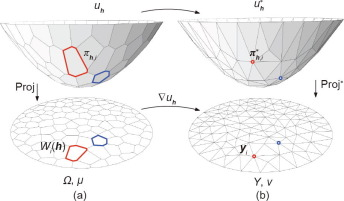
\includegraphics[width=0.6\linewidth]{6.jpg}
	\caption{分片线性Brenier势能函数(a)及其Legendre变换$u_h^*(b)$。$\pi_{h,n}^*$;$\pi_{h,i}$的Legendre对偶;$\bigtriangledown  : u_k$的梯度;Proj:投影映射;Proj*:Legendre对偶空间内的投影映射。}
	\label{fig:6}
\end{figure}

Brenier势能图是一个凸多面体。每个支撑平面$\pi_{h,i}$,i对应于多面体的一个面。多面体的投影诱导了$\Omega$的胞腔分解,其中每个支撑平面$\pi _i(x)$投射到一个胞胞$W_i(h),p$上是$\mathbb{R}^d$中的任意点:
\begin{equation}
	\Omega=\bigcup_{i=1}^{n} w_i(h) \cap \Omega, W_i(h)=\left \{ p \in \mathbb{R}^d \mid \bigtriangledown  u_h(p)=y_i \right \}  
	\label{function:20}
\end{equation}

胞腔分解是一个功率图。$W_i \cap \Omega$的$\mu$-测度记为$w_i(h)$:
\begin{equation}
	w_i(h)=\mu\left [ W_i(h) \cap \Omega \right ] = \int _{W_i(h) \cap \Omega}\mathrm{d}\mu  
	\label{function:21}
\end{equation}

梯度映射:$\bigtriangledown u_h : \Omega \to Y$将每个单元格$W_i(h)$映射到一个点$y_i$:
\begin{equation}
	\bigtriangledown u_h : W_i(h) \to y_i, i=1,2, \cdots ,n 
	\label{function:22}
\end{equation}

给定等式(\ref{function:17})中的目标度量$\nu$,在等式(\ref{function:19})中存在一个离散的布雷尼尔势,其每个面$w_i(h)$的投影$\mu$体积等于给定的目标度量$\nu _i$。 Alexandrov[46]在凸几何中证明了这一点。
\begin{theorem}[Alexandrov【46】] \label{theorem:4.1}
	假设$\Omega$是一个紧凑的凸多面体,在$\mathbb{R}^d$中内部为非空,$n_1,\cdots, n_k \subset \mathbb{R}^{n+1}$是不同的$k$个单位向量,$(n+1)$坐标为负,$v_1,\cdots, v_k > 0$,因此$\sum_{i=1}^{k} \nu _i= vol(\Omega)$ 。然后存在一个有精确$k$余维-1面$F_1, \cdots ,F_k$的凸多面体$P \subset \mathbb{R}^{n+1}$,其中$n_i$是$F_i$的法向量,并且在$\Omega$和$F_i$的投影之间有体积$v_i$。此外,这种$P$在垂直平移之前是唯一的。
	
	Alexandrov的解的存在性证明是基于代数拓扑,这不是构造性的。最近,Gu等人[6]提供了一个基于变分方法的构造性证明。
\end{theorem}

\begin{theorem}[参考文献【6】]\label{theorem:4.2}
	设$\mu$是定义在$\mathbb{R}^d$紧凸域$\Omega$上的概率测度,设$Y=\{ y_1,y_2,\cdots, y_n \}$是$\mathbb{R}^d$中的一个不同点。然后对于$\sum_{i=1}^n v_i=\mu(\Omega)$的任何$v_1,v_2,\cdots, v_n>0$,对于所有$i$,存在唯一的添加一个常数$(c,c,\cdots,c)$使得$w_i(h)=v_i$的$h=(h_1,h_2,\cdots, h_n)\in \mathbb{R}^n$。向量$\mathbf{h}$是以下凸能量的唯一最小值参数:
	\begin{equation}
		E(h) =\int_0^h \sum_{i=1}^n w_i(\eta)\mathrm{d}\eta_i  - \sum_{i=1}^n h_iv_i
		\label{function:23}
	\end{equation}

	定义在一个开的凸集上
	\begin{equation}
		H=\left \{ h\in \mathbb{R}^d : w_i(h)>0,i=1,2,\cdots ,n  \right \} 
		\label{function:24}
	\end{equation}

	此外,$\bigtriangledown u_k$使二次代价最小化
	\begin{equation}
		\frac{1}{2} \int_{\Omega} \left \| x-T(x) \right \|^2 \mathrm{d}\mu(x)
		\label{function:25}
	\end{equation}
	在所有的传输映射中,$T_{\# \mu} = \nu$。
	
	上述凸能量在等式(\ref{function:23})中的梯度值如下:
	\begin{equation}
		\bigtriangledown E(h)=\left [ w_1(h)-v_1, w_2(h)-v_2, \cdots , w_n(h)-v_n \right ]^T
		\label{function:26}
	\end{equation}

	能量的第$i$行和第$j$列元素如下:
	\begin{equation}
		\frac{\partial w_i}{\partial h_j} =-\frac{\mu (W_i \cap W_j \cap \Omega)}{\left \| y_i-y_j \right \| }, \frac{\partial w_i}{\partial h_i} = \sum_{j\ne i}\frac{\partial w_i}{\partial h_j} 
		\label{function:27}
	\end{equation}

	如图 \ref{fig:6} 所示,Hessian矩阵有一个明确的几何解释。图\ref{fig:6}(a)显示了离散的布雷尼尔势$u_h$,而图\ref{fig:6}(b)显示了其使用定义(\ref{definition:3.3})的勒让德变换。勒让德变换可以用几何方法构造:对于每个支撑平面$\pi_{h,i}$,我们构造对偶点$\pi_{h,i}^*$;对偶点的凸包$\{\pi_{h,1}^* ,\pi_{h,2}^* , \cdots , \pi_{h,n}^* \}$是勒让德变换的图$u_h^*$。
	
	$u_h^*$的投影得到了一个的三角剖分$Y=\{ y_1,y_2, \cdots ,y_n \}$,即加权的德劳内三角剖分。如图\ref{fig:7}所示,等式(\ref{function:20})中的能量图和加权的德劳内三角剖分是庞加莱对偶的:如果在幂图中,$W_i(h)$和$W_j(h)$在一个$(d-1)$-维胞腔上相交,那么在加权的德劳内三角剖分中,$y_i$与$y_j$连接。在等式(\ref{function:27})中的黑森矩阵的元素是能量图中$(d-1)$单元的$\mu$体积与加权德劳内三角剖分中双边的长度之间的比值。
\end{theorem}

传统的幂次图可以与上述定理密切相关。

\begin{figure}[h]
	\centering
	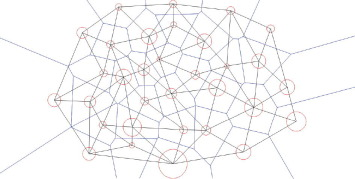
\includegraphics[width=0.6\linewidth]{7.jpg}
	\caption{Power diagram(蓝色)和其对偶加权Delaunay三角剖分(黑色)。}
	\label{fig:7}
\end{figure}


\begin{definition}[power距离]\label{definition:4.1}
	给定一个功率权重为$\psi _i$的点$y_i \in \mathbb{R}^d$,power距离如下:
	\begin{equation}
		pow(x,y_i)=\left \| x-y_i \right \|^2 -\psi _i
		\label{function:28}
	\end{equation}
\end{definition}

\begin{definition}[power图]\label{definition:4.2}
	给定加权点$(y_1,\psi _1), \cdots , (y_k, \psi _k)$,幂图为单元分解的$\mathbb{R}^d$:
	\begin{equation}
		\mathbb{R}^d=\bigcup_{i=1}^{k} W_i(\psi) 
		\label{function:29}
	\end{equation}
	其中,每个单元格都是一个凸多面体:
	\begin{equation}
		W_i(\psi)=\left \{ x \in \mathbb{R}^d \mid pow(x,y_j) \le pow(x,y_j) \right \} 
		\label{function:30}
	\end{equation}
	
	加权德劳内三角剖分,记为$T(\psi)$,是幂图的庞加莱对偶;如果$W_i(\psi)\cap W_j(\psi) \ne \phi$,那么在加权德劳内三角剖分中有一条边连接$y_i$和$y_j$。注意,$pow(x,y_i) \le pow(x,y_j)$等价于
	\begin{equation}
		\left \langle x,y_i \right \rangle +\frac{1}{2} (\psi _i -\left \| y_i \right \|^2 ) \ge \left \langle x,y_j \right \rangle + \frac{1}{2} (\psi _j -\left \| y_j \right \|^2 )
		\label{function:31}
	\end{equation}

	让$h_i=\frac{1}{2} (\psi _i - \left \| y_i \right \|^2 )$;然后我们将其定义重写如下:
	\begin{equation}
		W_i(\psi)=\left \{ x \in \mathbb{R}^d \mid \left \langle x,y_i \right \rangle +h_i \ge \left \langle x,y_j \right \rangle +h_j , \forall j \right \} 
		\label{function:32}
	\end{equation}
\end{definition}

在实践中,我们的目标是计算离散的布雷尼尔的潜在等式(\ref{function:19})通过优化凸能量等式(\ref{function:23}).对于低维情况,我们可以通过计算牛顿方法直接计算梯度等式(\ref{function:26})和黑森矩阵等式(\ref{function:27})。对于深度学习应用,直接计算黑森矩阵是不可行的;相反,我们可以使用梯度下降法或具有超线性收敛性的拟牛顿法。梯度的关键是估计$\mu$体积$w_i(h)$。这可以用蒙特卡罗方法来实现:我们从分布$µ$中抽取$n$个随机样本,并计算在$W_i(h)$范围内的样本数量,这是收敛于$\mu$体积的比值。这种方法是纯并行的,可以使用GPU来实现。此外,我们还可以使用分层的方法来进一步提高效率:首先,我们将目标样本分类为聚类,并计算到聚类质量中心的OT映射;其次,对于每个聚类,我们计算从相应的细胞到聚类内原始目标样本的OT映射。

\begin{figure}[h]
	\centering
	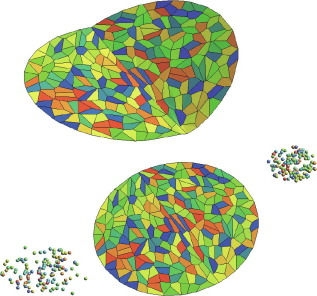
\includegraphics[width=0.6\linewidth]{8.jpg}
	\caption{Brenier势能函数的奇异点集与OT映射的间断点集。}
	\label{fig:8}
\end{figure}

为了避免模态坍塌,我们需要在$\Omega$中找到奇异点集。如图\ref{fig:8}所示,目标狄拉克测度有两个簇;源是单位平面圆盘上的均匀分布。布雷尼尔势函数的图是一个中间有一个脊的凸多面体。脊在圆盘上的投影是奇异集$\sum_1(u)$,最优映射在$\sum_1$上是不连续的。在一般情况下,如果两个单元格$W_i(h)$和$W_j(h)$相邻,则我们计算法线与相应支撑平面之间的夹角:
\begin{equation*}
	\theta _{ij} =\frac{\left \langle x_i,y_j \right \rangle }{\left \| y_i \right \| \left \| y_j \right \| } 
\end{equation*}

如果$\theta _{ij}$大于一个阈值,则公共面$W_i(h) \cap W_j(h)$在不连续奇异集合中。
% !TeX root = ../translation.tex

\section{GAN和最优传输}

OT理论为GANgan奠定了理论基础。许多最近的工作,如WGAN[1],WGAN-GP[27],和RW-GAN[47],使用瓦瑟斯坦距离来测量生成的数据分布和真实数据分布之间的偏差。

从OT的角度来看,生成器和鉴别器的最优解以一种封闭的形式联系起来;因此,生成器和鉴别器应该协作而不是竞争。更多细节请参见参考文献。[11].此外,Monge-Ampère解的正则性理论可以解释GAN[48]中的模态坍缩。

\subsection{竞争与合作}

WGAN[1]的OT视图如图 \ref{fig:2} 所示。根据流形分布假设,真实数据分布$\nu$接近于嵌入在环境空间$\chi $中的流形$\sum$。生成器计算从潜在空间$Z$到环境空间的解码映射$g_\theta$,并将白噪声$\zeta$(即高斯分布)转换为生成的分布$\mu _{\theta}$。该鉴别器通过计算坎托罗维奇的潜在$\varphi _{\zeta}$,计算$\mu _{\theta}$与真实数据分布$\nu$,$W_c(\mu _{\theta},\nu)$之间的瓦瑟斯坦距离。$g_{\theta}$和$\varphi _{\zeta}$都是由DNN实现的。

在训练过程中,生成器改善$g_{\theta}$通过$(g_{\theta})_{\#} \zeta$来更好地近似$\nu$;鉴别器改进了坎托洛维奇势$\varphi _{\zeta}$以改进对瓦瑟斯坦距离的估计。生成器和鉴别器相互竞争,而不共享中间的计算结果。在$L^1$成本函数下,WGAN的替代训练过程可以表述为期望的最小-最大优化:
\begin{equation*}
	\min_{\theta } \max_{\xi } E_{z\sim \zeta } \left \{ \varphi _{\xi } \left [ g_{\theta } (z) \right ]   \right \} + E_{y\sim \nu}\left [ \varphi_{\xi}^c (y) \right ]  
\end{equation*}

但如果我们将代价函数改变为$L^2$距离,那么根据定理(\ref{theorem:3.2}),在最优时,布雷尼尔的势$\mu$和康塔洛维奇的势$\varphi$通过等式(\ref{function:16})的封闭形式 $u(x)=\frac{1}{2} \left \| x \right \|^2 -\varphi(x)$ 联系起来, 生成器追求OT映射$\bigtriangledown u$;鉴别器计算$\varphi$。因此,一旦生成器达到最优值,无需任何训练就可以得到鉴别器的最优解,反之亦然。

更详细地说,假设在第$k$次迭代时,生成器映射为$g_{\theta}^k$。鉴别器计算康塔洛维奇势$\varphi_{\zeta}$,给出当前生成的数据分布$\left ( g_{\theta}^k \right )_{\#} \zeta $和真实数据分布$\nu$之间的瓦瑟斯坦距离;$\bigtriangledown u$给出从$\left ( g_{\theta}^k \right )_{\#} \zeta $到 $\nu$的OT映射。因此,我们得到了以下结果:
\begin{equation*}
	v=(\bigtriangledown u)_{\#} \left [ \left ( g_{\theta}^k \right )_{\#} \zeta \right ] =\left ( \bigtriangledown u\circ \left ( g_{\theta}^k \right )_{\#} \zeta \right )_{\#} \zeta =\left [ (id-\bigtriangledown _{\varphi _{\zeta}}) \circ g_{\theta}^k \right ] _{\#} \zeta
\end{equation*}

这意味着可以通过以下方式更新生成器映射:
\begin{equation}
	g_{\theta }^{k+1}=(id-\bigtriangledown \varphi _{\zeta }) \circ g_{\theta }^{k}
	\label{function:33}
\end{equation}

这一结论表明,原则上可以跳过发电机的训练过程;在实践中,通过共享中间的计算结果,可以大大提高效率。因此,在设计加纳人的架构时,协作优于竞争。

\subsection{模态崩溃与正则性}

虽然GAN对许多应用程序都很强大,但它们有关键的缺点:首先,GAN的训练很棘手,对超参数敏感,难以收敛;第二,GAN易产生模式崩溃;第三,GAN可能产生不真实的样本。不收敛、模态崩溃和生成不真实样本的问题都可以用OT映射的正则性定理(\ref{theorem:3.5})来解释。

根据布雷尼尔的极分解,定理(\ref{theorem:3.2}),任何保测度映射都可以分解为两个映射,其中一个是OT映射,它是Monge-Ampère方程的解。根据正则性定理(\ref{theorem:3.5}),如果目标测度$\nu$的支持$\Lambda$有多个连通分量——即如果$\nu$有多个模,或者$\Lambda$是非凸的,那么OT映射$T: \Omega \to \Lambda$在奇异集$\sum _{\Omega}$上是不连续的。

图\ref{fig:9} 显示了多簇的情况:$\Lambda$有两个连接的组件,其中OT映射$T$沿着$\sum_1$是不连续的。图\ref{fig:10}显示,即使是$\Lambda$也是连通的,尽管是非凸的。$\Omega$是一个矩形,$\Lambda$是一个哑铃形,密度函数是常数,OT映射是不连续的,奇异集$\sum_1 = \gamma_1 \cup \gamma_2$。

\begin{figure}[h]
	\centering
	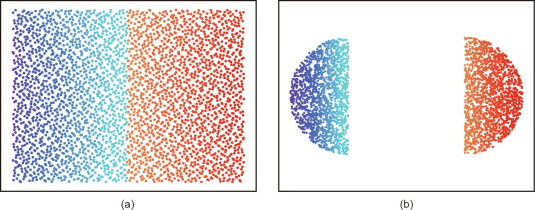
\includegraphics[width=0.6\linewidth]{9.jpg}
	\caption{不连续的OT映射,由基于Theorem\ref{theorem:4.2}的一个GPU算法实现生成。(a)源域;(b)目标域。(a)图中间的线代表的是奇异点集合$\sum_1$。}
	\label{fig:9}
\end{figure}

\begin{figure}[h]
	\centering
	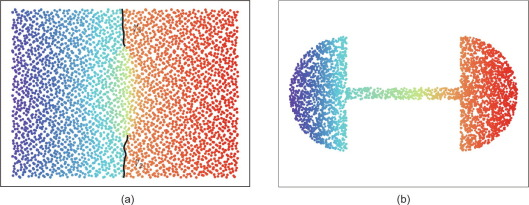
\includegraphics[width=0.6\linewidth]{10.jpg}
	\caption{不连续的OT映射,由基于Theorem \ref{theorem:4.2} 的一个GPU算法实现生成。(a)源域;(b)目标域。(a)图中的$\gamma_1$和$\gamma_2$是两个奇异点集合。}
	\label{fig:10}
\end{figure}

图\ref{fig:11}为$\mathbb{R}^3$中两个概率测度值之间的OT图。源测度$\mu$和目标测度$\nu$都是均匀分布;$\Omega$的支持是单位固体球,而$\Lambda
$的支持是固体斯坦福兔子。基于定理$\ref{theorem:4.2}$,我们计算了布雷尼尔势$u:\Omega \to \mathbb{R}$。为了可视化映射,我们插值概率测量如下:
\begin{equation*}
	\rho _t := \left [ (1-t)id+t\bigtriangledown \mu \right ]_{\#} \mu , 0 \le t \le 1 
\end{equation*}

图\ref{fig:11}为插值测量值$\rho_t$的支持度。表面上的折叠是奇点集,其中OT映射是不连续的。
\begin{figure}[h]
	\centering
	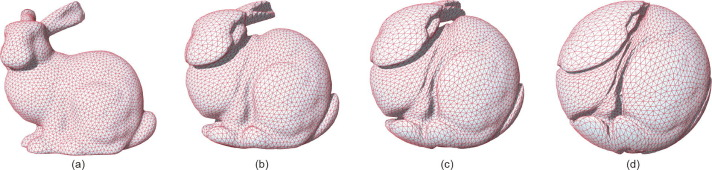
\includegraphics[width=0.6\linewidth]{11.jpg}
	\caption{从Stanford兔子到实心球的OT映射。边界曲面上的皱褶是奇异点集合。(a)~(d)显示了变化过程。}
	\label{fig:11}
\end{figure}

在一般情况下,由于真实数据分布、嵌入流形$\sum$和编码/解码映射的复杂性,目标测度量的支持度很少是凸的;因此,运输映射不能是全局连续的。

另一方面,一般的dnn,如ReLUdnn,只能近似于连续映射。由ReLUdnn表示的函数空间不包含所需的不连续传输映射。培训过程,或者,同样地,搜索过程将导致三种替代的情况:

(1) 训练过程不稳定,且不收敛。

(2) 搜索收敛于$\Lambda$的多个连通分量之一,并且映射收敛于所需的运输映射的一个连续分支。这意味着会遇到一个模式崩溃。

(3) 在培训过程中产生了一个交通地图,它成功地覆盖了所有的模式,但也覆盖了$\Lambda$以外的区域。在实际应用中,这将导致产生不现实的样本的现象,如图\ref{fig:12}的中间帧所示。
\begin{figure}[h]
	\centering
	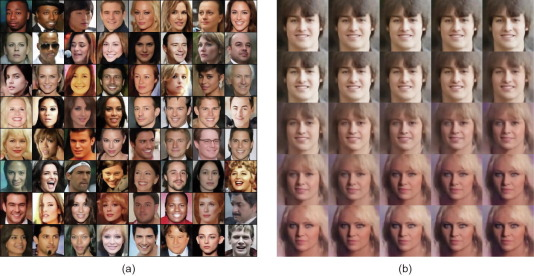
\includegraphics[width=0.6\linewidth]{12.jpg}
	\caption{AE-OT模型生成的人脸图像。(a)生成的实际人脸图像;(b)经过奇异点的路径。(b)图中心位置处的图像的传输映射是非连续的。}
	\label{fig:12}
\end{figure}


因此,在理论上,不可能直接使用DNN来近似OT映射。

\subsection{AE-OT模型}

如图\ref{fig:4}所示,我们分离了GANs的两个主要任务:流形学习和概率分布变换。第一个任务由AE执行,计算编码/解码映射$f_{\theta}, g_{\zeta}$;第二个任务是使用显式变分方法来计算潜在空间中的OT映射$T$。真实的数据分布v由编码映射$f_{\theta}$向前推进,诱导$(f_{\theta})_{\#} \nu$。在潜在空间中,$T$将均匀分布$\mu$映射到$(f_{\theta})_{\#} \nu$。

AE-OT模型有许多优点。在本质上,寻找OT映射是一个凸优化问题;保证了解的存在性和唯一性。采用拟牛顿方法,训练过程稳定且具有超线性收敛性。未知数的数量等于训练样本的数量,避免了过度参数化。并行OT映射算法可以使用GPU来实现。用蒙特卡罗方法可以通过采样密度来控制OT图的误差界。具有自适应能力的分层算法进一步提高了算法的效率。特别是,AE-OT模型可以消除模式崩溃。
% !TeX root = ../translation.tex

\section{试验结果}

在本节中,我们将报告我们的实验结果

\subsection{训练过程}

AE-OT模型的训练主要包括两个步骤:训练AE和寻找OT图。OT步骤是使用该算法的GPU实现来完成的,如第4节所述。在AE步骤中,在训练过程中,我们采用Adam算法[49]对中性网络的参数进行优化,学习速率为$0.003,\beta_1=0.5,\beta_2=0.999$。当$L^2$损失停止下降时,这意味着网络已经找到了一个良好的编码图,我们冻结编码器部分,并继续训练网络进行解码图。编码器冻结前后的训练损失见表(\ref{table:1})。接下来,为了从给定的分布(这里使用均匀分布)到潜在特征的分布中找到OT映射,我们从均匀分布中随机抽取$100N$个随机点来计算能量的梯度。这里,$N$是数据集的潜在特征的数量。此外,在实验中,$\theta_{ij}$被设置为对不同的数据集的不同。具体来说,对于MNIST和Fashion-MNIST数据集,$\theta_{ij}$被设置为$0.75$,而对于CIFAR-10和CelebA数据集,它分别被设置为$0.68$和$0.75$。
\begin{table}[!htbp]
	\caption{编码器冻结前后AEs的$L^2$损失}
	\label{table:1}
	\centering
	\begin{tabular}{@{}ccccc@{}}
		\toprule
		\multirow{2}{*}{Situation} & \multicolumn{4}{c}{Dataset}                \\ \cmidrule(l){2-5} 
		& MNIST  & Fashion-MNIST & CIFAR-10 & CelebA \\ \cmidrule(r){1-5}
		Before                     & 0.0013 & 0.0026        & 0.0023   & 0.0077 \\
		After                      & 0.0005 & 0.0011        & 0.0018   & 0.0074 \\ \bottomrule
	\end{tabular}
\end{table}

我们的AE-OT模型是在一个Linux平台上使用PyTorch实现的。所有实验均在GTX1080Ti上进行。

\subsection{传输映射的不连续性试验}

在这个实验中,我们想要检验我们的假设:在大多数实际应用中,目标测度的支持是非凸的,奇异集是非空的,概率分布映射沿奇异集是不连续的。

如图\ref{fig:12}所示,我们使用AE计算从CelebA数据集$(\sum,\nu)$到潜在空间Z的编码/解码映射;编码映射$f_{\theta}: \sum \to Z$在潜在空间上将$\nu$向前推到$(f_{\theta})_{\#}\mu$。在潜在空间中,我们基于第4节,$T: Z\to Z$中描述的算法计算OT映射,其中$T$将单位立方体$\zeta$中的均匀分布映射到$(f_{\theta})_{\#}\nu$。然后,我们从分布$\zeta$中随机抽取一个样本$z$,并使用解码映射$g_{\xi}:Z\to \sum$ 将$T(z)$映射到生成的人类面部图像$g_{\xi} \circ T(z)$。图\ref{fig:12}(a)展示了由该AE-OT框架生成的真实面部图像。

如果潜在空间中的推进测度$(f_{\theta})_{\#} \nu$的支持是非凸的,则会有一个奇异集$\sum _k$,其中$k>0$。我们想检测出$\sum _k$的存在。我们在潜在空间中随机抽取单位立方体中的线段,然后沿着这条线段进行密集插值,生成面部图像。如图\ref{fig:12}(b)所示,我们找到了一个线段$\gamma$,并在一个有一双棕色眼睛的男孩和一个有一对蓝眼睛的女孩之间生成了一个变形序列。在中间,我们生成了一张有一只蓝眼睛和一只棕色眼睛的脸,这绝对是不现实的,而且在$\sum$之外。这个结果意味着线段$\gamma$经过一个奇异集$\sum _k$,其中运输图$T$是不连续的。这也表明了我们的假设是正确的:编码的人脸图像测量在潜在空间上的支持是非凸的。

作为一个副产品,我们发现这个AE-OT框架提高了训练速度的5倍,并提高了收敛稳定性,因为OT步骤是一个凸优化。因此,它为改进现有的GAN提供了一种很有前途的方法。

\subsection{模式崩溃比较}

由于合成数据集由显式分布和已知模态组成,因此可以准确地测量模态坍塌。我们选择了两个在之前的工作中研究或提出的合成数据集:一个二维网格数据集。

为了选择模态崩溃的测量度量,我们采用了三个以前使用的度量[50,51]。模式的数量计算由生成模型产生的样本所捕获的模式的数量。在这个度量中,如果在该模式的三个标准差内没有产生样本,则被认为是丢失的。高质量样本的百分比衡量在最近模式的三个标准差内产生的样本的比例。第三个度量标准,在参考文献中使用。[51],是反向回-莱布勒(KL)散度。在这个度量中,每个生成的样本被分配到其最近的模式,并且我们计算分配在每个模式上的样本的直方图。然后,该直方图形成一个离散分布,然后计算其与真实数据形成的直方图的KL散度。直观地说,这衡量了生成的样本在真实分布的所有模式之间的平衡程度

在参考文献中。[51],作者用上述三个指标评估了GAN[26]、ALI[52]、MD[30]和PacGAN[51]。每个实验都在相同的生成器架构下进行训练,总共有大约400k的训练参数。这些网络在100k个样本上被训练了400个时代。对于AE-OT实验,由于源空间和目标空间都是二维的,因此不需要训练AE。我们直接计算了一个半离散的OT,它映射在单位平方上的均匀分布和经验的真实数据分布之间。理论上,OT恢复所有模式所需的最小真实样本量是每个模式一个样本。然而,这可能会导致在插值过程中产生低质量的样品。因此,对于OT计算,我们取512个真实样本,并基于此映射生成新的样本。我们注意到,在这种情况下,在OT计算中只有512个参数需要优化,并且由于凸正定黑森的存在,优化过程是稳定的。我们的结果在表(\ref{table:2})中所示,以前的方法的基准测试是从参考文献中复制出来的。[51]为了说明这一点,我们在图\ref{fig:13}中绘制了与GAN和PAcGAN一起绘制的合成数据集上的结果。
\begin{table}[!htbp]
	\caption{二维网格数据集的模式折叠比较}
	\label{table:2}
	\centering
	\begin{tabular}{@{}cccc@{}}
		\toprule
		& Modes       & Samples       & Reverse KL     \\ \midrule
		GAN     & 17.3\pm 0.8  & 94.8 \pm 0.7\% & 0.70 \pm 0.07   \\
		ALI     & 24.1 \pm 0.4 & 95.7 \pm 0.6\% & 0.14 \pm 0.03   \\
		MD      & 23.8 \pm 0.5 & 79.9 \pm 3.2\% & 0.17 \pm 0.003  \\
		PacGAN2 & 23.8 \pm 0.7 & 91.3 \pm 0.8\% & 0.13 \pm 0.04   \\
		PacGAN3 & 24.6 \pm 0.4 & 94.2 \pm 0.4\% & 0.06 \pm 0.02   \\
		PacGAN4 & 24.8 \pm 0.2 & 93.6 \pm 0.6\% & 0.04 \pm 0.01   \\
		AE-OT   & 25.0 \pm 0.0 & 99.8 \pm 0.2\% & 0.007 \pm 0.002 \\ \bottomrule
	\end{tabular}
\end{table}

\begin{figure}[h]
	\centering
	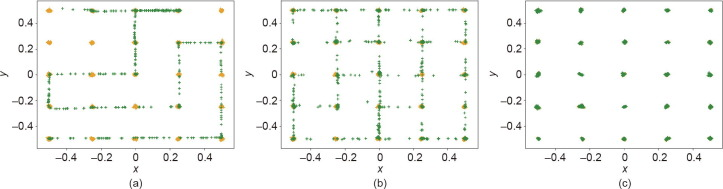
\includegraphics[width=0.6\linewidth]{13.jpg}
	\caption{2D格点数据集上的模式崩溃比较。(a)GAN;(b)PacGAN4;(c)AE-OT。橙色点代表真实样本,绿色点代表生成样本。}
	\label{fig:13}
\end{figure}

\subsection{与现有技术水平的比较}

我们设计了实验来比较我们提出的AE-OT模型与最先进的生成模型,包括由Lucic等人评估的对抗性模型。[33],以及Hoshen和Malik研究的非对抗性模型。[36].

为了进行公平的比较,我们使用了相同的测试数据集和网络体系结构。这些数据集包括MNIST[53]、MNIST-Dashion[54]、CIFAR-10[55]和CelebA[56],与在Refs中测试的数据类似。[31,36].该网络架构与Lucic等人在参考文献中使用的类似。[33].特别是,在我们的AE-OT模型中,解码器的网络结构与Ref中GANs的生成器相同。[33],编码器与解码器对称。

我们使用FID评分[31]和PRD曲线作为评价标准,将我们的模型与最先进的生成模型进行了比较。FID评分衡量生成结果的视觉保真度,并对图像损坏具有鲁棒性。然而,FID评分对模式的添加和删除[33]很敏感。因此,我们也使用了PRD曲线,它可以量化真实数据集[32]上的模式下降程度。

\subsubsection{与FID评分的比较}

FID得分的计算方法如下:\textcircled{1} 通过运行初始网络[30]提取生成的图像和真实图像在视觉上有意义的特征;\textcircled{2} 用高斯分布拟合真实和生成的特征分布;\textcircled{3} 使用以下公式计算两个高斯分布之间的距离:
\begin{equation}
	FID = \left \| u_r - u_g \right \|_2^2 + T_r \left [ \sum_r + \sum_g - 2\left ( \sum_r \sum_g \right )^{\frac{1}{2} }  \right ] 
	\label{function:34}
\end{equation}
其中,$\mu _r$和$\mu _g$分别表示真实分布和生成分布的平均值;$\sum _r$和$\sum _g$表示这些分布的方差

比较结果汇总见表(\ref{table:3})和表(\ref{table:4})。各种GANs的统计数据来自Lucic等人的[33],而非对抗性生成模型的统计数据来自Hoshen和Malik[36]。总的来说,我们提出的模型比其他最先进的生成模型获得了更好的FID分数。
\begin{table}[!htbp]
	\caption{与FID-I进行的定量比较}
	\label{table:3}
	\centering
	\begin{tabular}{@{}cclccl@{}}
		\toprule
		\multirow{2}{*}{Dataset} & \multicolumn{5}{c}{Adversarial}                 \\ \cmidrule(l){2-6} 
		& MM GAN & NS GAN & LS GAN & WGAN & BEGAN         \\ \cmidrule(r){1-6}
		MNIST                    & 9.8    & 6.8    & 7.8    & 6.7  & 13.1          \\
		Fashion-MNIST            & 29.6   & 26.5   & 30.7   & 21.5 & 22.9          \\
		CIF AR-10                & 72.7   & 58.5   & 87.1   & 55.2 & 71.4          \\
		CelebA                   & 65.6   & 55.0   & 53.8   & 41.3 & \textbf{38.9} \\ \bottomrule
	\end{tabular}
\end{table}

最佳结果以粗体显示。

\begin{table}[!htbp]
	\caption{与FID-II之间的定量比较}
	\label{table:4}
	\centering
	\begin{tabular}{@{}ccccccc@{}}
		\cmidrule(r){1-7}
		\multirow{2}{*}{Dataset} & \multicolumn{3}{c}{Non-adversarial} &  & \multicolumn{2}{c}{Reference} \\ \cmidrule(lr){2-4} \cmidrule(l){6-7} 
		& VAE        & GLO       & CLANN      &  & AE        & AE-OT             \\ \cmidrule(r){1-7}
		MNIST                    & 23.8       & 49.6      & 8.6        &  & 5.5       & \textbf{6.4}      \\
		Fashion-MNIST            & 58.7       & 57.7      & 13.0       &  & 4.7       & \textbf{10.2}     \\
		CIF AR-10                & 155.7      & 65.4      & 46.5       &  & 28.2      & \textbf{38.1}     \\
		CelebA                   & 85.7       & 52.4      & 46.3       &  & 67.5      & 68.4(\textbf{28.6})        \\ \cmidrule(r){1-7}
	\end{tabular}
\end{table}

最佳结果以粗体显示。

理论上,我们的AE-OT模型的FID分数应该与预先训练过的AEs模型的分数很接近;我们的实验也验证了这一点。

我们的AE的固定网络架构采用了Lucic等人的[33];它的容量不足以编码CIFAR-10或CelebaA,所以我们不得不对这些数据集进行降采样。我们从CIFAR-10中随机选择25k图像,从CelebA中选择10k图像来训练我们的模型。即便如此,我们的模型在CIFAR-10中获得了最好的FID分数。由于InfoGAN模型的有限容量,CelebA的AE性能的FID为67.5并不理想,进一步导致生成的数据集的FID为68.4。通过在AE体系结构中增加两个卷积层,CelebA的$L^2$损失小于$0.03$,FID得分优于其他所有的模型($28.6$,如表(\ref{table:4})的括号所示)。

\begin{figure}[h]
	\centering
	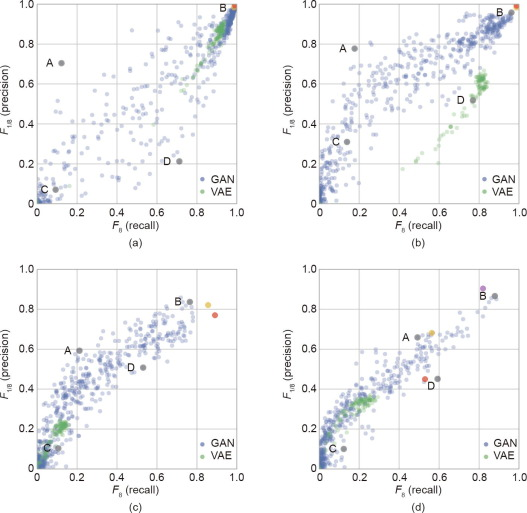
\includegraphics[width=0.6\linewidth]{14.jpg}
	\caption{在四个数据集上,以(F8, F1/8)的精确度-召回率进行比较。(a)MNIST;(b)FASHION;(c)CIFAR-10;(d)CelebA。黄褐色的点表示参考文献[36]中的结果。红色的点是利用本文所提出的方法生成的结果。(d)中紫色的点代表添加两个卷积层后,利用本文所提出的方法生成的结果。}
	\label{fig:14}
\end{figure}

\subsubsection{与PRD曲线的比较}

FID评分是衡量生成分布与真实数据分布差异的有效方法,但它主要关注精度,不能准确地捕获生成模型可以覆盖的真实数据的哪个部分。参考文献中提出的方法。[32]将分布之间的差异分解为两个组成部分:精度和召回率。

给定一个参考分布P和一个学习到的分布$Q$,精度直观地衡量从$Q$中获得的样本的质量,而召回率则衡量$Q$所覆盖的$P$的比例。

我们使用了Sajjadi等人在参考文献中提出的($F_8$,$F_{1 \setminus  8}$)的概念。[32]来量化精度和查全率的相对重要性。图\ref{fig:14}总结了比较结果。每个点代表一个具有一组超参数的特定模型。一个点越靠近右上角,模型的性能就越好。蓝色和绿色的点表示参考文献中评估的GANs和VAEs。[32],黄点代表Ref中的GLANN模型。[36],红点是我们的AE-OT模型.

很明显,我们提出的模型在MNIST和Dashion-MNIST上优于其他模型。对于CIFAR-10数据集,我们的模型的精度略低于GANs和GLANN,但查全率最高。对于CelebA数据集,由于AE的容量有限,我们的模型的性能并不令人印象深刻。然而,在AE中增加了两个卷积层后,我们的模型获得了最好的分数。

\subsubsection{视觉比较}

图\ref{fig:15}显示了我们提出的方法生成的图像与Lucic等人研究的GAN生成的图像之间的视觉比较。[33]和Hoshen和Malik研究的非对抗性模型。[36].第一列显示了原始图像,第二列显示了AE生成的结果,第三列显示最好的生成结果的差距在Lucicetal.[33],第四列显示所生成的结果霍申和马利克[36]的模型,和第五列显示我们的方法的结果。很明显,我们的方法可以生成高质量的图像,并覆盖了所有的模式。

\begin{figure}[h]
	\centering
	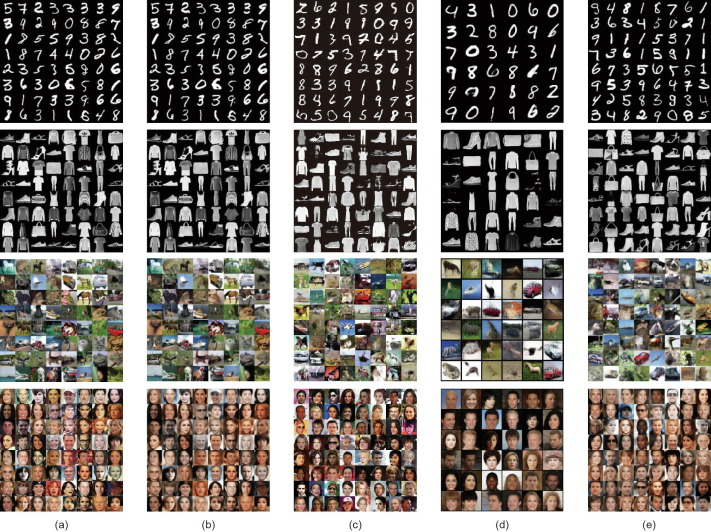
\includegraphics[width=0.6\linewidth]{15.jpg}
	\caption{生成图像质量在 4 个数据集上的可视化比较。第一列(a)是真实数据;第二列(b)是由AE生成的结果;第三列(c)显示的是由GAN[33]以最高的精确度-查全率$(F_8,F_{1 \setminus 8})$生成的结果,它对应着图\ref{fig:14}中的B点;第四列(d)是参考文献[36]中的结果;最后一列(e)是利用本文所提出的方法生成的结果。}
	\label{fig:15}
\end{figure}
% !TeX root = ../translation.tex

\section{结论}

这项工作使用OT理论来解释gan。根据数据流形分布假设,GANs主要完成两个任务:流形学习和概率分布变换。后一种任务可以直接使用OT方法来完成。这一理论理解解释了模态崩溃的根本原因,并表明了发生器和鉴别器之间的内在关系应该是协作,而不是竞争。此外,我们提出了一个AE-OT模型,它提高了理论的严密性、训练的稳定性和效率,并消除了模式崩溃。

我们的实验验证了我们的假设,即如果分布运输图是不连续的,那么奇点集的存在会导致模态崩溃。此外,当我们提出的模型与现有的技术进行比较时,我们的方法消除了模态崩溃,并在FID评分和PRD曲线方面优于其他模型。

在未来,我们将探索对流形学习阶段的理论理解,并使用一种严格的方法来使黑盒的这一部分透明。
% !TeX root = ../translation.tex

\section*{致谢}

该项目部分由国家自然科学基金会(61936002,61772105,61432003,617201060005,61772379),美国国家科学基金会CMMI-1762287合作研究:计算框架设计适形伸缩电子,福特URP拓扑优化细胞中间结构的非线性行为碰撞安全,和美国国家科学基金会DMS-1737812合作研究:ATD:从人类移动和监测网络数据离散曲率的理论和算法。

%-------------------------------------------------------
% References
% !TeX root = ../translation.tex

\section*{参考文献}



%-------------------------------------------------------
% Appendix
% % !TeX root = ../thuthesis-example.tex

\chapter{补充内容}

附录是与论文内容密切相关、但编入正文又影响整篇论文编排的条理和逻辑性的资料,例如某些重要的数据表格、计算程序、统计表等,是论文主体的补充内容,可根据需要设置。


\section{图表示例}

\subsection{图}

附录中的图片示例(图~\ref{fig:appendix-figure})。

\begin{figure}
  \centering
  
\includegraphics[width=0.6\linewidth]{example-image-a.pdf}
  \caption{附录中的图片示例}
  \label{fig:appendix-figure}
\end{figure}


\subsection{表格}

附录中的表格示例(表~\ref{tab:appendix-table})。

\begin{table}
  \centering
  \caption{附录中的表格示例}
  \begin{tabular}{ll}
    \toprule
    文件名          & 描述                         \\
    \midrule
    thuthesis.dtx   & 模板的源文件,包括文档和注释 \\
    thuthesis.cls   & 模板文件                     \\
    thuthesis-*.bst & BibTeX 参考文献表样式文件    \\
    thuthesis-*.bbx & BibLaTeX 参考文献表样式文件  \\
    thuthesis-*.cbx & BibLaTeX 引用样式文件        \\
    \bottomrule
  \end{tabular}
  \label{tab:appendix-table}
\end{table}


\section{数学公式}

附录中的数学公式示例(公式\eqref{eq:appendix-equation})。
\begin{equation}
  \frac{1}{2 \uppi \symup{i}} \int_\gamma f = \sum_{k=1}^m n(\gamma; a_k) \mathscr{R}(f; a_k)
  \label{eq:appendix-equation}
\end{equation}


\includepdf[pages=-]{A Geometric Understanding of Deep Learning.pdf}

\end{document}
